\subsection{Qualitative Case Examples}
\label{app:qualitative-cases}
To illustrate the interaction pattern enabled by A2UI, we present four qualitative examples as shown in Figure~\ref{fig:appendix_case_1}--\ref{fig:appendix_case_4}, spanning motivational interviewing, emotional support, and task-oriented assistance. Each figure keeps only the dialogue context that is needed to interpret the final turn, together with the assistant's last utterance and the rendered interface, so that the dialogue-to-UI handoff remains easy to inspect.

\begin{figure}[t]
\centering
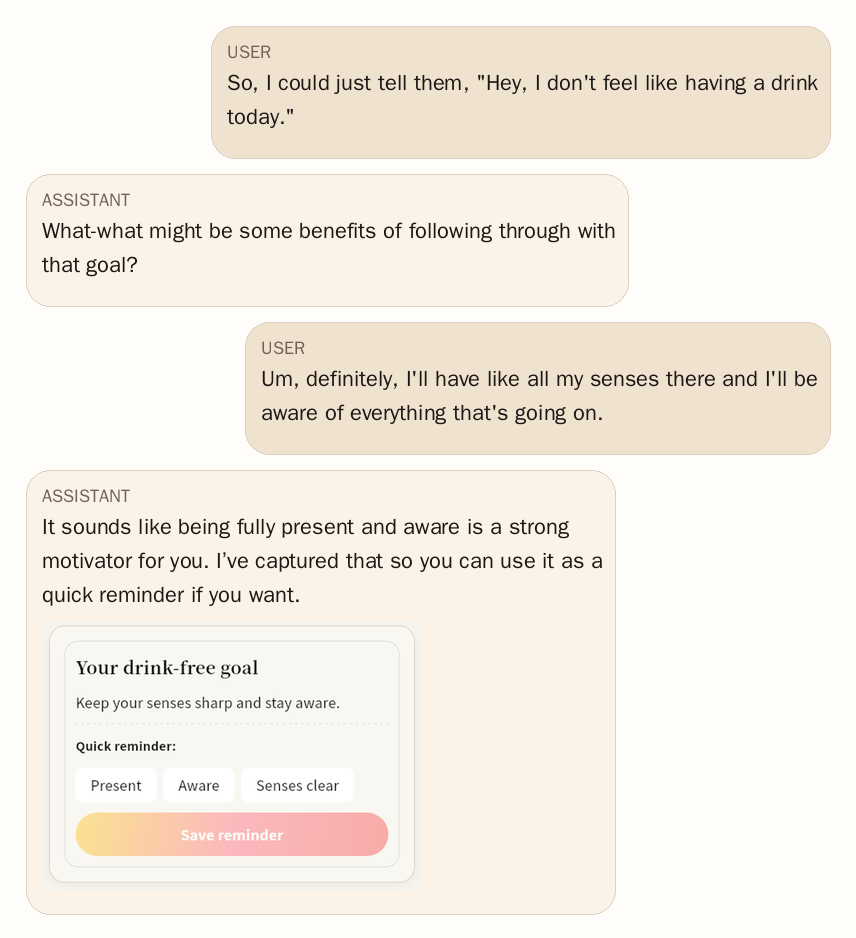
\includegraphics[width=0.86\linewidth]{Figures/appendix_case_panels/004_atomic_annomi_ce91cccc.png}
\caption{A reflective motivational exchange culminates in a concise reminder card that turns an abstract goal into a concrete next step.}
\label{fig:appendix_case_1}
\end{figure}

\begin{figure}[t]
\centering
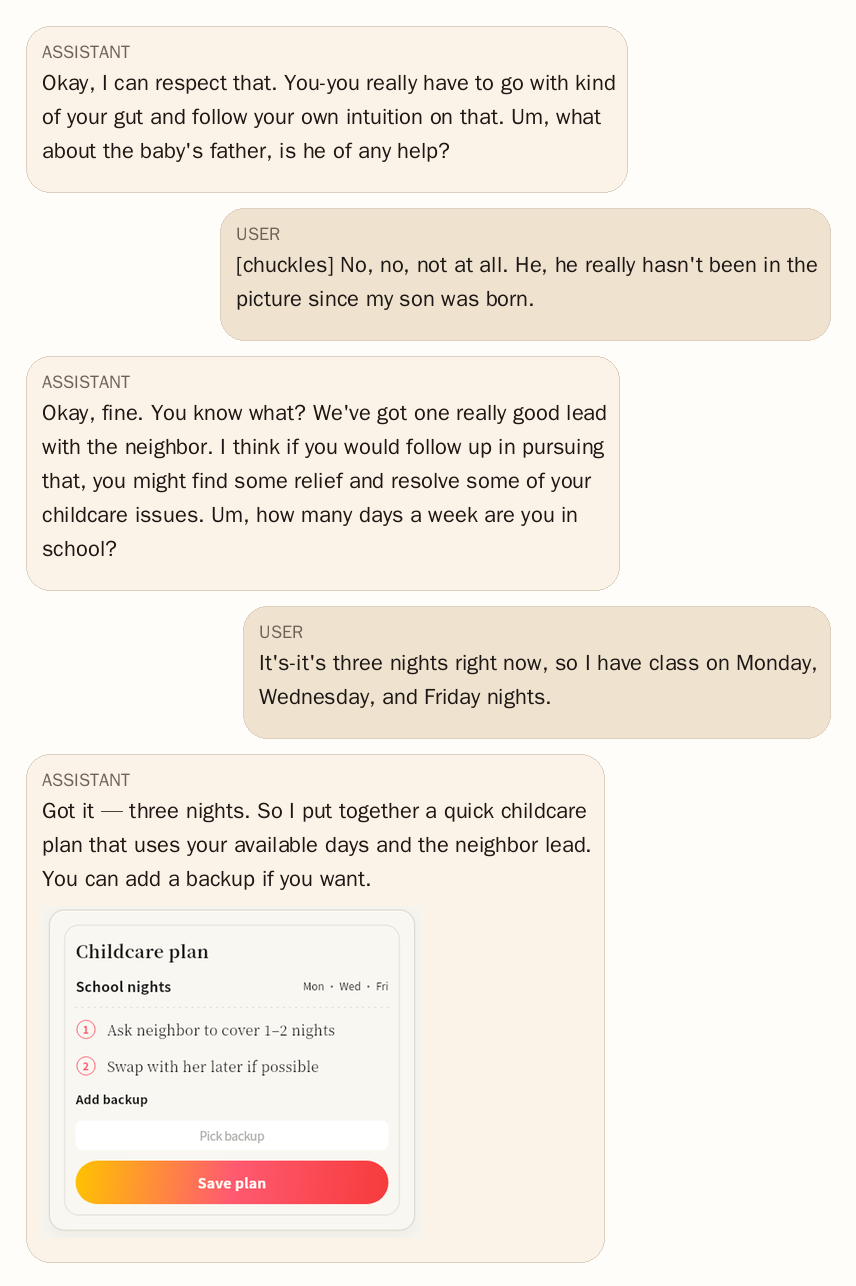
\includegraphics[width=0.86\linewidth]{Figures/appendix_case_panels/001_atomic_annomi_00b81ae7.png}
\caption{The assistant distills a long discussion about childcare logistics into a lightweight planning card with immediately actionable options.}
\label{fig:appendix_case_2}
\end{figure}

\begin{figure}[t]
\centering
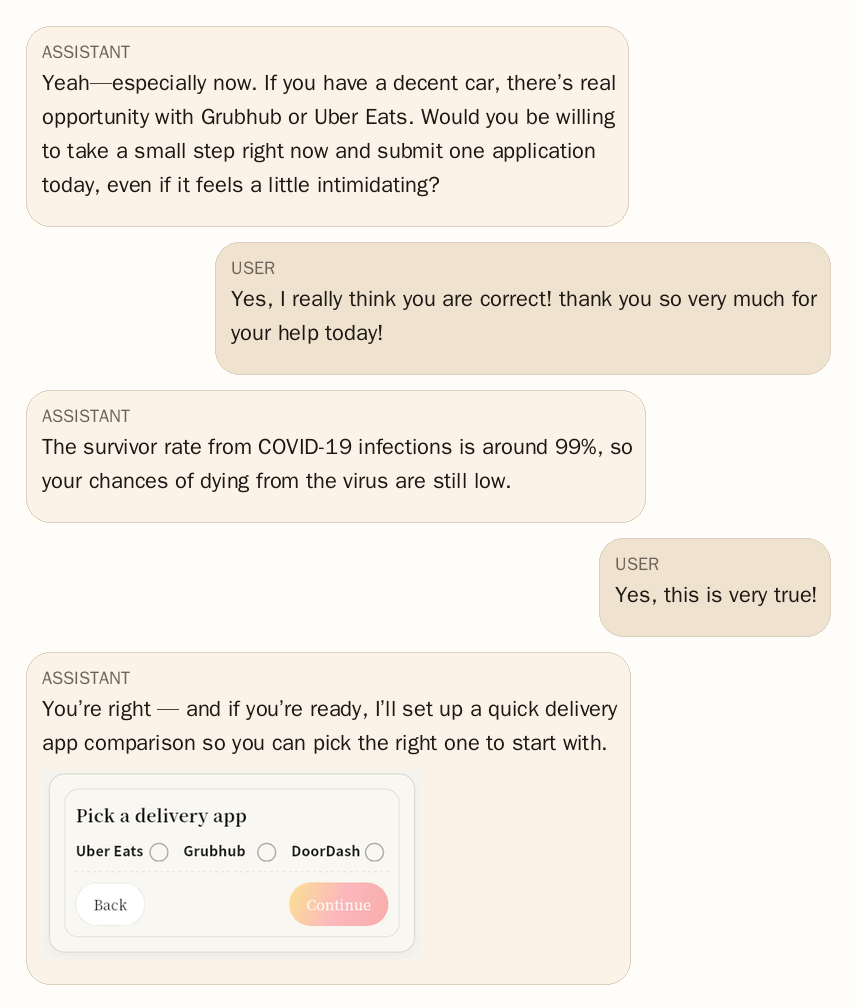
\includegraphics[width=0.86\linewidth]{Figures/appendix_case_panels/015_atomic_esconv_7c66d172.png}
\caption{A supportive counseling exchange is resolved with a compact decision card, reducing cognitive load at the point of action.}
\label{fig:appendix_case_3}
\end{figure}

\begin{figure}[t]
\centering
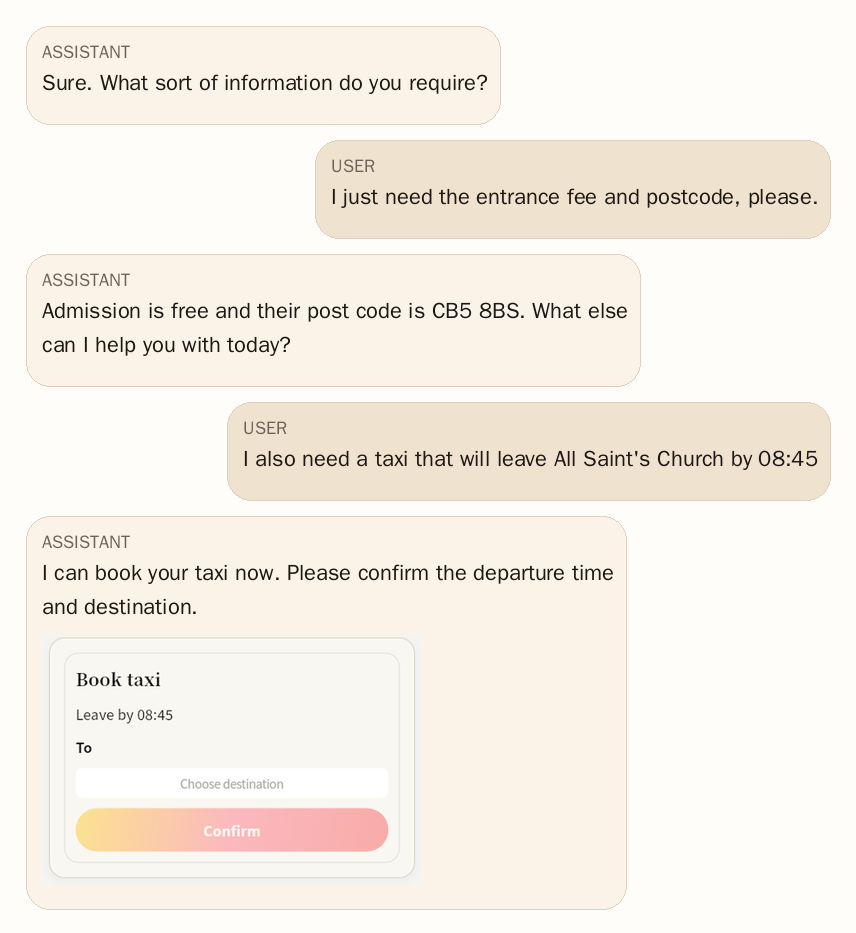
\includegraphics[width=0.86\linewidth]{Figures/appendix_case_panels/049_atomic_multiwoz_70b48c8c.png}
\caption{The final booking turn is rendered as a compact confirmation surface, making the transaction state easy to verify at a glance.}
\label{fig:appendix_case_4}
\end{figure}
